\documentclass[10pt]{article}
\usepackage[margin=0.8in]{geometry}
\usepackage{amsmath,amssymb,booktabs,graphicx}
\title{Supplementary Material: Decision-Threshold Selection and Zero-Noise Extrapolation}
\date{}
\begin{document}
\maketitle
\renewcommand{\thetable}{S\arabic{table}}
This document accompanies the main manuscript. The supplementary tables contain secondary unstandardized-PCA exact and finite grids, cross-task contrasts, channel and error controls, clipping and allocation diagnostics, scale sensitivity, a separate weak-signal synthetic diagnostic, calibration-size sensitivity, standardized-PCA noise results, depth score-spread diagnostics, and transfer comparisons. Supplementary Figures S1--S3 show secondary unstandardized-PCA diagnostics. Except where stated otherwise, results reuse saved outer folds and are descriptive.

\section*{Secondary unstandardized-PCA and paired analyses}

\begin{table}[t]
\centering
\caption{Secondary unstandardized-PCA WDBC exact-expectation results (mean across saved model runs).}
\label{tab:exact}
\scriptsize
\setlength{\tabcolsep}{2.2pt}
\resizebox{\textwidth}{!}{%
\begin{tabular}{@{}rccccccccc@{}}
\toprule
$\gamma$ & Fixed & Fixed AUC & Clean-frozen & Noisy-calibrated & Affine & Linear ZNE & Quadratic ZNE & Linear ZNE+cal. & Quadratic ZNE+cal. \\
\midrule
0.00 & 0.812 & 0.959 & -- & 0.885 & 0.875 & -- & -- & -- & -- \\
0.05 & 0.809 & 0.959 & -- & 0.886 & 0.875 & -- & -- & -- & -- \\
0.10 & 0.792 & 0.959 & 0.560 & 0.886 & 0.872 & 0.821 & 0.816 & 0.886 & 0.886 \\
0.15 & 0.726 & 0.958 & -- & 0.886 & 0.872 & -- & -- & -- & -- \\
0.20 & 0.606 & 0.958 & 0.527 & 0.886 & 0.872 & 0.849 & 0.835 & 0.886 & 0.886 \\
0.25 & 0.537 & 0.958 & -- & 0.886 & 0.872 & -- & -- & -- & -- \\
0.30 & 0.500 & 0.958 & 0.526 & 0.886 & 0.872 & 0.626 & 0.837 & 0.886 & 0.886 \\
0.35 & 0.500 & 0.958 & -- & 0.885 & 0.872 & -- & -- & -- & -- \\
0.40 & 0.500 & 0.958 & 0.500 & 0.885 & 0.872 & 0.538 & 0.606 & 0.885 & 0.885 \\
\bottomrule
\end{tabular}}
\end{table}

\begin{table}[t]
\centering
\caption{Secondary unstandardized-PCA finite-shot WDBC balanced accuracy (mean $\pm$ SD over model and shot repetitions), AUC, collapse frequency, and total measurements. The clean-frozen threshold requires a clean calibration measurement and is a simulator-only reference.}
\label{tab:finite}
\scriptsize
\begin{tabular}{@{}r r l c c c r@{}}
\toprule
$\gamma$ & Budget/test case & Method & Balanced accuracy & AUC & Collapse rate & Total shots \\
\midrule
0.30 & 1000 & Affine readout & 0.749 $\pm$ 0.056 & 0.828 & 0.000 & 113809 \\
0.30 & 1000 & Noisy-calibrated threshold & 0.755 $\pm$ 0.049 & 0.828 & 0.000 & 113809 \\
0.30 & 1000 & Clean-frozen threshold & 0.524 $\pm$ 0.058 & 0.828 & 0.750 & 113809 \\
0.30 & 1000 & Fixed threshold & 0.500 $\pm$ 0.000 & 0.874 & 1.000 & 113800 \\
0.30 & 1000 & Linear ZNE & 0.611 $\pm$ 0.072 & 0.830 & 0.000 & 113800 \\
0.30 & 1000 & Linear ZNE + calibration & 0.690 $\pm$ 0.042 & 0.778 & 0.000 & 113809 \\
0.30 & 1000 & Quadratic ZNE & 0.617 $\pm$ 0.045 & 0.664 & 0.000 & 113800 \\
0.30 & 1000 & Quadratic ZNE + calibration & 0.575 $\pm$ 0.041 & 0.620 & 0.000 & 113809 \\
\bottomrule
\end{tabular}
\end{table}

\begin{table}[t]
\centering
\caption{Secondary unstandardized-PCA cross-task and broader-input finite-shot balanced accuracy at $\gamma=0.30$ and 1,000 shots per test case. Each calibration-based method includes calibration measurements; realized totals differ from the fixed-threshold comparator by at most 0.443\%.}
\label{tab:transfer}
\begin{tabular}{@{}l c c c c c@{}}
\toprule
Task and circuit & Fixed clean BA ($\gamma=0$) & Noisy calibration & Linear ZNE & Linear ZNE+cal. & Quadratic ZNE+cal. \\
\midrule
WDBC, 2q CNOT & 0.812 & 0.755 & 0.611 & 0.690 & 0.575 \\
WDBC, 4q CNOT star & 0.838 & 0.509 & 0.503 & 0.506 & 0.495 \\
Wine, 2q CNOT & 0.850 & 0.684 & 0.627 & 0.626 & 0.550 \\
Balanced synthetic, 2q CNOT & 0.697 & 0.620 & 0.605 & 0.599 & 0.528 \\
\bottomrule
\end{tabular}
\end{table}

\begin{table}[t]
\centering
\caption{WDBC fixed-threshold channel controls across saved primary-model runs.}
\label{tab:channels}
\begin{tabular}{@{}l r c c c r@{}}
\toprule
Channel & $\gamma$ & Balanced accuracy & ROC-AUC & Collapse rate & Model runs \\
\midrule
amplitude\_damping & 0.20 & 0.763 & 0.960 & 0.000 & 10 \\
amplitude\_damping & 0.30 & 0.644 & 0.961 & 0.500 & 10 \\
amplitude\_damping & 0.40 & 0.611 & 0.962 & 0.500 & 10 \\
composite & 0.20 & 0.606 & 0.958 & 0.600 & 10 \\
composite & 0.30 & 0.500 & 0.958 & 1.000 & 10 \\
composite & 0.40 & 0.500 & 0.958 & 1.000 & 10 \\
depolarizing & 0.20 & 0.818 & 0.957 & 0.000 & 10 \\
depolarizing & 0.30 & 0.817 & 0.956 & 0.000 & 10 \\
depolarizing & 0.40 & 0.818 & 0.956 & 0.000 & 10 \\
phase\_damping & 0.20 & 0.818 & 0.957 & 0.000 & 10 \\
phase\_damping & 0.30 & 0.820 & 0.957 & 0.000 & 10 \\
phase\_damping & 0.40 & 0.821 & 0.956 & 0.000 & 10 \\
\bottomrule
\end{tabular}
\end{table}

\begin{table}[t]
\centering
\caption{Observable error for WDBC at $\gamma=0.30$ and 1,000 shots per test case. Exact RMSE is relative to the clean observable; sampling RMSE is deviation from the exact method-specific observable. Calibration-rule fitting uncertainty and classification performance are reported separately.}
\label{tab:errors}
\begin{tabular}{@{}l c c@{}}
\toprule
Method & Exact observable RMSE & Finite sampling RMSE \\
\midrule
Noisy-calibrated threshold & 0.595 & 0.042 \\
Clean-frozen threshold & 0.595 & 0.042 \\
Fixed threshold & 0.595 & 0.030 \\
Linear ZNE & 0.683 & 0.086 \\
Linear ZNE + calibration & 0.683 & 0.120 \\
Quadratic ZNE & 0.576 & 0.471 \\
Quadratic ZNE + calibration & 0.576 & 0.681 \\
\bottomrule
\end{tabular}
\end{table}

\begin{table}[t]
\centering
\caption{Direct paired contrasts for ZNE minus calibration.}
\label{tab:paired}
\scriptsize
\begin{tabular}{@{}l r r l l r c r@{}}
\toprule
$\gamma$ & Analysis & Shots & Reference & ZNE & Difference & Descriptive 95\% interval & Folds \\
\midrule
0.20 & finite-shot & 100 & Noisy-calibrated threshold & Linear ZNE & -0.012 & [-0.031, +0.006] & 5 \\
0.20 & finite-shot & 100 & Noisy-calibrated threshold & Linear ZNE + calibration & -0.064 & [-0.090, -0.034] & 5 \\
0.20 & finite-shot & 100 & Noisy-calibrated threshold & Quadratic ZNE & -0.139 & [-0.167, -0.114] & 5 \\
0.20 & finite-shot & 100 & Noisy-calibrated threshold & Quadratic ZNE + calibration & -0.165 & [-0.202, -0.122] & 5 \\
0.20 & finite-shot & 1000 & Noisy-calibrated threshold & Linear ZNE & -0.029 & [-0.054, -0.006] & 5 \\
0.20 & finite-shot & 1000 & Noisy-calibrated threshold & Linear ZNE + calibration & -0.027 & [-0.046, -0.008] & 5 \\
0.20 & finite-shot & 1000 & Noisy-calibrated threshold & Quadratic ZNE & -0.129 & [-0.143, -0.112] & 5 \\
0.20 & finite-shot & 1000 & Noisy-calibrated threshold & Quadratic ZNE + calibration & -0.201 & [-0.213, -0.191] & 5 \\
0.30 & finite-shot & 100 & Noisy-calibrated threshold & Linear ZNE & +0.002 & [-0.006, +0.012] & 5 \\
0.30 & finite-shot & 100 & Noisy-calibrated threshold & Linear ZNE + calibration & -0.019 & [-0.048, +0.011] & 5 \\
0.30 & finite-shot & 100 & Noisy-calibrated threshold & Quadratic ZNE & -0.050 & [-0.076, -0.024] & 5 \\
0.30 & finite-shot & 100 & Noisy-calibrated threshold & Quadratic ZNE + calibration & -0.057 & [-0.090, -0.024] & 5 \\
0.30 & finite-shot & 1000 & Noisy-calibrated threshold & Linear ZNE & -0.144 & [-0.171, -0.122] & 5 \\
0.30 & finite-shot & 1000 & Noisy-calibrated threshold & Linear ZNE + calibration & -0.065 & [-0.094, -0.040] & 5 \\
0.30 & finite-shot & 1000 & Noisy-calibrated threshold & Quadratic ZNE & -0.138 & [-0.179, -0.110] & 5 \\
0.30 & finite-shot & 1000 & Noisy-calibrated threshold & Quadratic ZNE + calibration & -0.180 & [-0.195, -0.167] & 5 \\
0.40 & finite-shot & 100 & Noisy-calibrated threshold & Linear ZNE & +0.001 & [-0.030, +0.035] & 5 \\
0.40 & finite-shot & 100 & Noisy-calibrated threshold & Linear ZNE + calibration & -0.004 & [-0.038, +0.034] & 5 \\
0.40 & finite-shot & 100 & Noisy-calibrated threshold & Quadratic ZNE & -0.008 & [-0.034, +0.025] & 5 \\
0.40 & finite-shot & 100 & Noisy-calibrated threshold & Quadratic ZNE + calibration & -0.008 & [-0.026, +0.015] & 5 \\
0.40 & finite-shot & 1000 & Noisy-calibrated threshold & Linear ZNE & -0.078 & [-0.094, -0.064] & 5 \\
0.40 & finite-shot & 1000 & Noisy-calibrated threshold & Linear ZNE + calibration & -0.047 & [-0.064, -0.030] & 5 \\
0.40 & finite-shot & 1000 & Noisy-calibrated threshold & Quadratic ZNE & -0.051 & [-0.068, -0.030] & 5 \\
0.40 & finite-shot & 1000 & Noisy-calibrated threshold & Quadratic ZNE + calibration & -0.072 & [-0.088, -0.055] & 5 \\
\bottomrule
\end{tabular}
\end{table}

\begin{table}[t]\centering\scriptsize
\caption{Transfer-setting paired contrasts at $\gamma=0.30$ and 1,000 nominal shots per test case. Differences are ZNE balanced accuracy minus noisy-calibrated-threshold balanced accuracy; intervals are descriptive bootstrap intervals over five fold-level means.}
\label{tab:transferpaired}
\begin{tabular}{@{}l l r l r@{}}\toprule
Task and circuit & Method & Difference & Descriptive 95\% interval & Folds \\
\midrule
Balanced synthetic, 2-qubit CNOT & Linear ZNE & -0.014 & [-0.027, -0.003] & 5 \\
Balanced synthetic, 2-qubit CNOT & Quadratic ZNE & -0.060 & [-0.075, -0.045] & 5 \\
WDBC, 2-qubit CNOT & Linear ZNE & -0.144 & [-0.171, -0.122] & 5 \\
WDBC, 2-qubit CNOT & Quadratic ZNE & -0.138 & [-0.179, -0.110] & 5 \\
WDBC, 4-qubit CNOT star & Linear ZNE & -0.006 & [-0.021, +0.008] & 5 \\
WDBC, 4-qubit CNOT star & Quadratic ZNE & -0.011 & [-0.032, +0.010] & 5 \\
Wine, 2-qubit CNOT & Linear ZNE & -0.057 & [-0.097, -0.008] & 5 \\
Wine, 2-qubit CNOT & Quadratic ZNE & -0.089 & [-0.125, -0.057] & 5 \\
\bottomrule\end{tabular}\end{table}

\begin{table}[t]\centering\scriptsize
\caption{Finite-shot ZNE with and without clipping scores to the Pauli-$Z$ interval, at $\gamma=0.30$ and 1,000 nominal shots per test case.}
\label{tab:zne_range}
\begin{tabular}{@{}l l r r r r@{}}\toprule
Task and circuit & Method & Raw BA & Clipped BA & Fraction outside $[-1,1]$ & Total shots \\
\midrule
Balanced synthetic, 2-qubit CNOT & Linear ZNE + calibration & 0.599 & 0.599 & 0.000 & 120000 \\
Balanced synthetic, 2-qubit CNOT & Quadratic ZNE + calibration & 0.528 & 0.528 & 0.168 & 120000 \\
WDBC, 2-qubit CNOT & Linear ZNE + calibration & 0.690 & 0.690 & 0.000 & 113809 \\
WDBC, 2-qubit CNOT & Quadratic ZNE + calibration & 0.575 & 0.575 & 0.175 & 113809 \\
WDBC, 4-qubit CNOT star & Linear ZNE + calibration & 0.506 & 0.506 & 0.000 & 113809 \\
WDBC, 4-qubit CNOT star & Quadratic ZNE + calibration & 0.495 & 0.494 & 0.159 & 113809 \\
Wine, 2-qubit CNOT & Linear ZNE + calibration & 0.626 & 0.626 & 0.000 & 35598 \\
Wine, 2-qubit CNOT & Quadratic ZNE + calibration & 0.550 & 0.559 & 0.168 & 35598 \\
\bottomrule\end{tabular}\end{table}

\begin{table}[t]\centering\scriptsize
\caption{Exploratory calibration-share sensitivity at WDBC, two-qubit CNOT chain, $\gamma=0.30$.}
\label{tab:allocation}
\begin{tabular}{@{}r l c r@{}}\toprule
Calibration share & Pipeline & Balanced accuracy & Mean total shots \\
\midrule
25\% & Noisy-calibrated threshold & 0.762 $\pm$ 0.057 & 113804 \\
25\% & Linear ZNE + calibration & 0.689 $\pm$ 0.065 & 113804 \\
25\% & Quadratic ZNE + calibration & 0.583 $\pm$ 0.047 & 113804 \\
50\% & Noisy-calibrated threshold & 0.753 $\pm$ 0.060 & 113809 \\
50\% & Linear ZNE + calibration & 0.691 $\pm$ 0.049 & 113809 \\
50\% & Quadratic ZNE + calibration & 0.584 $\pm$ 0.056 & 113809 \\
75\% & Noisy-calibrated threshold & 0.711 $\pm$ 0.053 & 113790 \\
75\% & Linear ZNE + calibration & 0.640 $\pm$ 0.050 & 113790 \\
75\% & Quadratic ZNE + calibration & 0.568 $\pm$ 0.060 & 113790 \\
\bottomrule\end{tabular}\end{table}

\begin{table}[t]\centering\scriptsize
\caption{Exploratory ZNE probability-scale sensitivity at WDBC, two-qubit CNOT chain, $\gamma=0.30$.}
\label{tab:scales}
\begin{tabular}{@{}l l l c c@{}}\toprule
Schedule & Scales & Richardson coefficients & Balanced accuracy & Observable RMSE \\
\midrule
1\_1p25 & 1.0;1.25 & 5;-4 & 0.697 & 0.629 \\
1\_1p25\_1p5 & 1.0;1.25;1.5 & 15;-24;10 & 0.855 & 0.497 \\
1\_1p5 & 1.0;1.5 & 3;-2 & 0.664 & 0.656 \\
\bottomrule\end{tabular}\end{table}

\begin{table}[t]\centering\small
\caption{Post-hoc finite-shot scale sensitivity at WDBC, $\gamma=0.30$, and 1,000 nominal measurements per test case. Entries are mean balanced accuracy $\pm$ SD over 10 checkpoints and two shot repetitions; training sets share observations.}
\label{tab:finite-scales}
\begin{tabular}{@{}l r r@{}}\toprule
Schedule & Fixed threshold & Calibration \\
\midrule
Linear $\{1,2\}$ & 0.615 $\pm$ 0.065 & 0.704 $\pm$ 0.055 \\
Mild $\{1,1.25\}$ & 0.620 $\pm$ 0.052 & 0.609 $\pm$ 0.055 \\
Mild $\{1,1.25,1.5\}$ & 0.527 $\pm$ 0.052 & 0.532 $\pm$ 0.048 \\
Mild $\{1,1.5\}$ & 0.625 $\pm$ 0.053 & 0.644 $\pm$ 0.062 \\
Quadratic $\{1,1.5,2\}$ & 0.576 $\pm$ 0.062 & 0.570 $\pm$ 0.055 \\
\bottomrule\end{tabular}\end{table}

\clearpage
\section*{Separate fresh-data synthetic diagnostic}

The diagnostic used 6 development realizations and 30 distinct held-out realizations (15 at class separations 0.9 and 15 at 1.2), generated afresh from the same balanced synthetic task family (500 examples, eight features, four informative and two redundant features, 2% label flips). A two-qubit, two-layer readout-centered CNOT-star circuit was trained without noise and evaluated with the composite simulator channel at $\gamma=0.30$. The development-only choice was the quadratic\_1\_1.25\_1.5 scale schedule and 75% calibration allocation at 1,000 nominal measurements per validation example; both were frozen before evaluating held-out realizations at 100 and 1,000 measurements per test case. One finite-shot draw was used per realization and budget. This diagnostic used Python 3.12.10, PennyLane 0.45.1, NumPy 2.2.6, pandas 2.3.3, and scikit-learn 1.9.0, distinct from the primary run environment, and is reported as a separate execution rather than a bitwise reproduction.

\begin{table}[t]\centering\small
\caption{Fresh synthetic transfer diagnostic at two nominal measurement budgets; the fixed-threshold results near 0.5 indicate weak discrimination, so this is not confirmatory evidence for the WDBC result. ZNE settings were selected on separate development data; ``cal.'' denotes threshold fitting on calibration labels. Mean and SD are over 30 generated datasets, with one shot draw per condition.}
\label{tab:fresh-diagnostic}
\begin{tabular}{@{}r l r r r@{}}\toprule
Budget & Pipeline & Mean BA & SD & $n$ \\
\midrule
100 & Fixed & 0.513 & 0.019 & 30 \\
100 & Noisy threshold & 0.516 & 0.052 & 30 \\
100 & ZNE (dev) & 0.514 & 0.058 & 30 \\
100 & ZNE (dev) + cal. & 0.508 & 0.043 & 30 \\
1000 & Fixed & 0.500 & 0.000 & 30 \\
1000 & Noisy threshold & 0.559 & 0.045 & 30 \\
1000 & ZNE (dev) & 0.519 & 0.048 & 30 \\
1000 & ZNE (dev) + cal. & 0.511 & 0.050 & 30 \\
\bottomrule\end{tabular}\end{table}

\begin{table}[t]\centering\scriptsize
\caption{Paired contrasts for the fresh synthetic diagnostic. Positive values favor noisy threshold selection. SD is across the 30 realization-level paired differences; intervals are descriptive percentile bootstraps over those realizations.}
\label{tab:confirm-paired}
\begin{tabular}{@{}r l r r l r@{}}\toprule
Budget & Contrast & Mean & SD & Descriptive 95\% interval & $n$ \\
\midrule
100 & Noisy threshold $-$ ZNE dev. & 0.002 & 0.059 & [-0.019, 0.023] & 30 \\
100 & Noisy threshold $-$ ZNE dev. + cal. & 0.008 & 0.064 & [-0.015, 0.030] & 30 \\
100 & Noisy threshold $-$ Fixed & 0.003 & 0.043 & [-0.013, 0.018] & 30 \\
1000 & Noisy threshold $-$ ZNE dev. & 0.040 & 0.067 & [0.016, 0.064] & 30 \\
1000 & Noisy threshold $-$ ZNE dev. + cal. & 0.049 & 0.057 & [0.028, 0.068] & 30 \\
1000 & Noisy threshold $-$ Fixed & 0.059 & 0.045 & [0.043, 0.075] & 30 \\
\bottomrule\end{tabular}\end{table}

This fresh task-family diagnostic is not a confirmation of the WDBC headline: the fixed pipeline is at chance and discrimination is weak. At 1,000 measurements, noisy threshold selection has the largest observed mean, 0.559, while development-selected ZNE is 0.519 and ZNE plus calibration is 0.511; at 100 measurements all four means are near chance. These descriptive results do not establish population-level superiority. The accompanying tables report the pipeline means and paired contrasts. Per-realization metrics, intermediate scores, checkpoints, and split indices are included in the run archive.

A candidate score-gap rule predicted a median of 11376 shots per calibration example, but its prespecified two-percentage-point regret criterion was met within the tested grid in only 3 of 30 held-out realizations. This is a negative, simulator-dependent result, not a validated budget predictor; exact simulated expectations used by the rule are unavailable on hardware.

\clearpage
\section*{Standardized-PCA sensitivity analyses}

\begin{table}[t]\centering\scriptsize
\caption{Post-hoc calibration-size sensitivity for standardized-PCA WDBC at $\gamma=0.30$. Each pipeline uses the same nominal total of 1,000 measurements per test case, with half allocated to calibration and half to test inference; finite-shot test scores are reused across calibration-size conditions. Shot draws are averaged within each of 10 checkpoints; means and SDs are across checkpoint means nested in five folds with shared training observations.}
\label{tab:calsize}
\begin{tabular}{@{}l r r r r@{}}\toprule
Method & Calibration labels & Balanced accuracy & AUC & Rows \\ \midrule
Linear ZNE & 10 & 0.709 $\pm$ 0.011 & 0.799 & 10 \\
Linear ZNE & 20 & 0.715 $\pm$ 0.013 & 0.799 & 10 \\
Linear ZNE & 50 & 0.716 $\pm$ 0.012 & 0.799 & 10 \\
Linear ZNE & 114 & 0.712 $\pm$ 0.013 & 0.799 & 10 \\
Noisy threshold & 10 & 0.760 $\pm$ 0.014 & 0.868 & 10 \\
Noisy threshold & 20 & 0.772 $\pm$ 0.012 & 0.868 & 10 \\
Noisy threshold & 50 & 0.779 $\pm$ 0.014 & 0.868 & 10 \\
Noisy threshold & 114 & 0.783 $\pm$ 0.010 & 0.868 & 10 \\
Quadratic ZNE & 10 & 0.596 $\pm$ 0.008 & 0.633 & 10 \\
Quadratic ZNE & 20 & 0.591 $\pm$ 0.007 & 0.633 & 10 \\
Quadratic ZNE & 50 & 0.591 $\pm$ 0.007 & 0.633 & 10 \\
Quadratic ZNE & 114 & 0.591 $\pm$ 0.008 & 0.633 & 10 \\
\bottomrule\end{tabular}\end{table}

\begin{table}[t]\centering\scriptsize
\caption{Exact-expectation composite-noise grid for the standardized-PCA WDBC primary checkpoints. Calibrated methods use thresholds selected on held-out calibration labels. Means and SDs are over 10 saved model checkpoints. Reconciliation from saved per-example scores gives 0.878 for the primary calibrated-threshold result at $\gamma=0.30$; the 0.891 entry here is fixed-threshold performance at $\gamma=0.10$, a different condition. The cause of the earlier summary mismatch is not established.}
\label{tab:stdnoise}
\begin{tabular}{@{}r l r r r@{}}\toprule
Noise $\gamma$ & Method & Balanced accuracy & AUC & Models \\ \midrule
0.0 & fixed\_threshold & 0.887 $\pm$ 0.035 & 0.958 & 10 \\
0.0 & linear\_zne\_calibrated & 0.882 $\pm$ 0.027 & 0.958 & 10 \\
0.0 & noisy\_threshold & 0.882 $\pm$ 0.027 & 0.958 & 10 \\
0.0 & quadratic\_zne\_calibrated & 0.882 $\pm$ 0.027 & 0.958 & 10 \\
0.1 & fixed\_threshold & 0.891 $\pm$ 0.035 & 0.958 & 10 \\
0.1 & linear\_zne\_calibrated & 0.880 $\pm$ 0.026 & 0.958 & 10 \\
0.1 & noisy\_threshold & 0.882 $\pm$ 0.026 & 0.958 & 10 \\
0.1 & quadratic\_zne\_calibrated & 0.881 $\pm$ 0.028 & 0.958 & 10 \\
0.2 & fixed\_threshold & 0.835 $\pm$ 0.041 & 0.959 & 10 \\
0.2 & linear\_zne\_calibrated & 0.880 $\pm$ 0.024 & 0.959 & 10 \\
0.2 & noisy\_threshold & 0.882 $\pm$ 0.025 & 0.959 & 10 \\
0.2 & quadratic\_zne\_calibrated & 0.881 $\pm$ 0.024 & 0.958 & 10 \\
0.3 & fixed\_threshold & 0.500 $\pm$ 0.000 & 0.958 & 10 \\
0.3 & linear\_zne\_calibrated & 0.883 $\pm$ 0.028 & 0.958 & 10 \\
0.3 & noisy\_threshold & 0.878 $\pm$ 0.027 & 0.958 & 10 \\
0.3 & quadratic\_zne\_calibrated & 0.884 $\pm$ 0.028 & 0.958 & 10 \\
0.4 & fixed\_threshold & 0.500 $\pm$ 0.000 & 0.958 & 10 \\
0.4 & linear\_zne\_calibrated & 0.876 $\pm$ 0.030 & 0.958 & 10 \\
0.4 & noisy\_threshold & 0.876 $\pm$ 0.030 & 0.958 & 10 \\
0.4 & quadratic\_zne\_calibrated & 0.884 $\pm$ 0.027 & 0.958 & 10 \\
\bottomrule\end{tabular}\end{table}

\begin{table}[t]\centering\scriptsize
\caption{Supplementary depth and score-separation diagnostic for standardized-PCA WDBC.}
\label{tab:depth}
\begin{tabular}{@{}r r r r r r r r r@{}}\toprule
Layers & Clean BA & Exact noisy BA & Finite BA $\pm$ SD & Finite AUC & Score SD & Class gap & SE at 500 & SE/gap \\ \midrule
1 & 0.873 & 0.849 & 0.854 $\pm$ 0.031 & 0.929 & 0.132 & 0.210 & 0.043 & 0.206 \\
2 & 0.887 & 0.878 & 0.778 $\pm$ 0.014 & 0.868 & 0.047 & 0.079 & 0.044 & 0.558 \\
4 & 0.885 & 0.873 & 0.525 $\pm$ 0.007 & 0.549 & 0.005 & 0.008 & 0.043 & 5.136 \\
\bottomrule\end{tabular}\end{table}

\begin{table}[t]\centering\scriptsize
\caption{Full standardized-PCA transfer comparison on the same saved splits and seeds.}
\label{tab:stdtransfer}
\begin{tabular}{@{}l r r r r@{}}\toprule
Task & Fixed threshold & Noisy threshold + calibration & Linear ZNE + calibration & Quadratic ZNE + calibration \\ \midrule
WDBC (standardized PCA) & 0.503 & 0.778 & 0.716 & 0.582 \\
Wine, class 0 vs rest & 0.500 & 0.701 & 0.650 & 0.557 \\
Synthetic, balanced & 0.500 & 0.612 & 0.584 & 0.534 \\
\bottomrule\end{tabular}\end{table}


\clearpage
\section*{Supplementary Figures}
\renewcommand{\thefigure}{S\arabic{figure}}
\begin{figure*}[t]
\centering
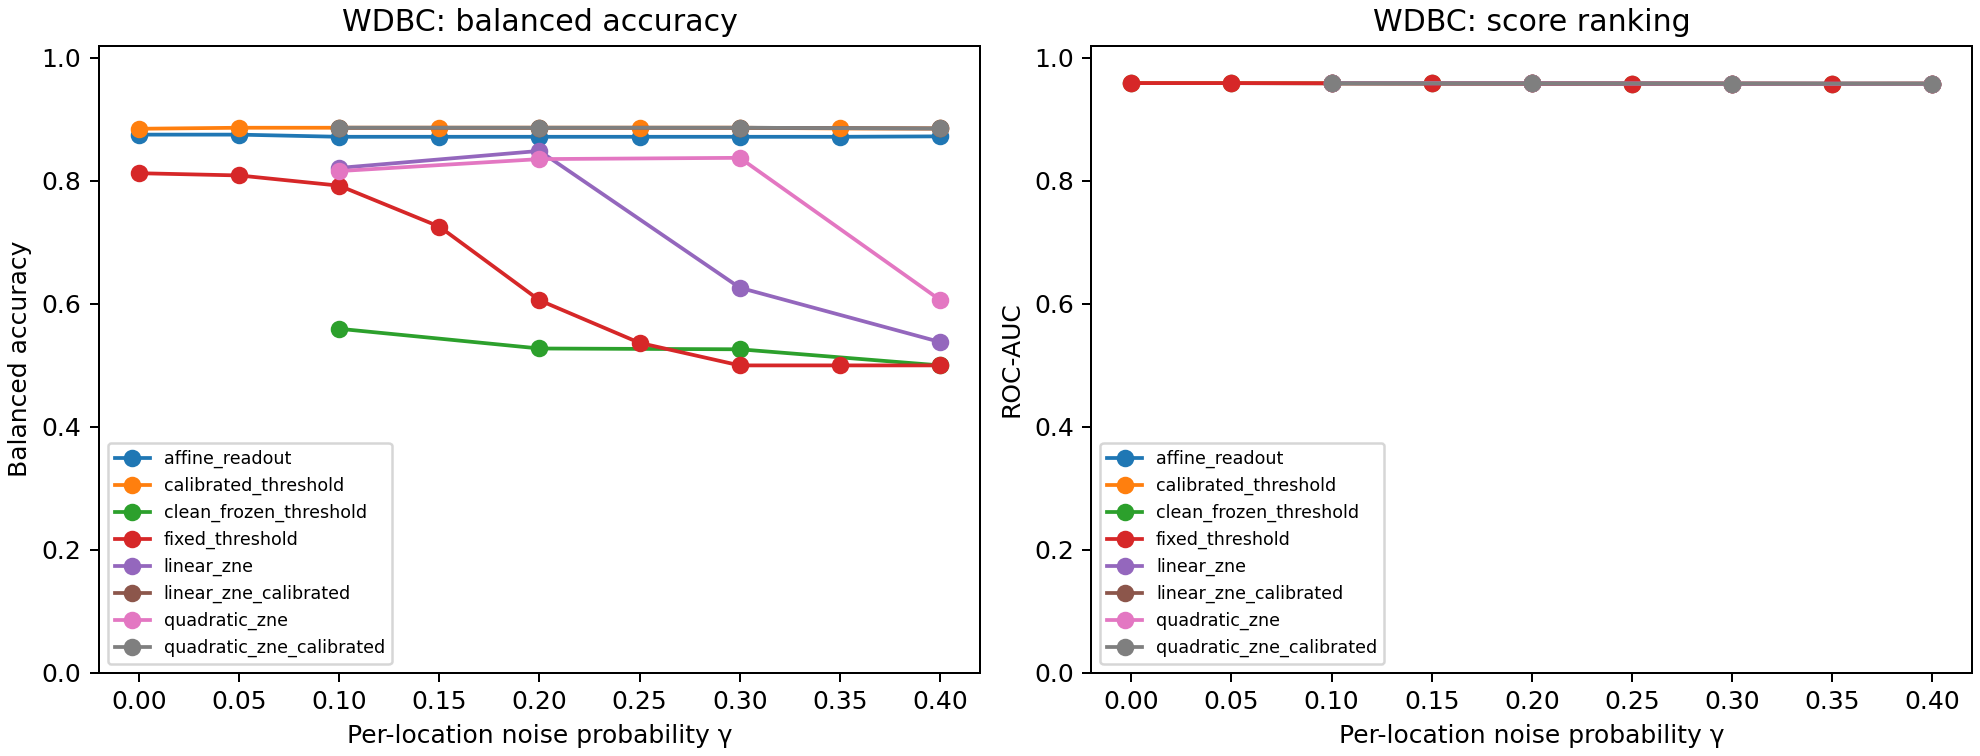
\includegraphics[width=0.48\textwidth]{exact_accuracy_auc.png}\hfill
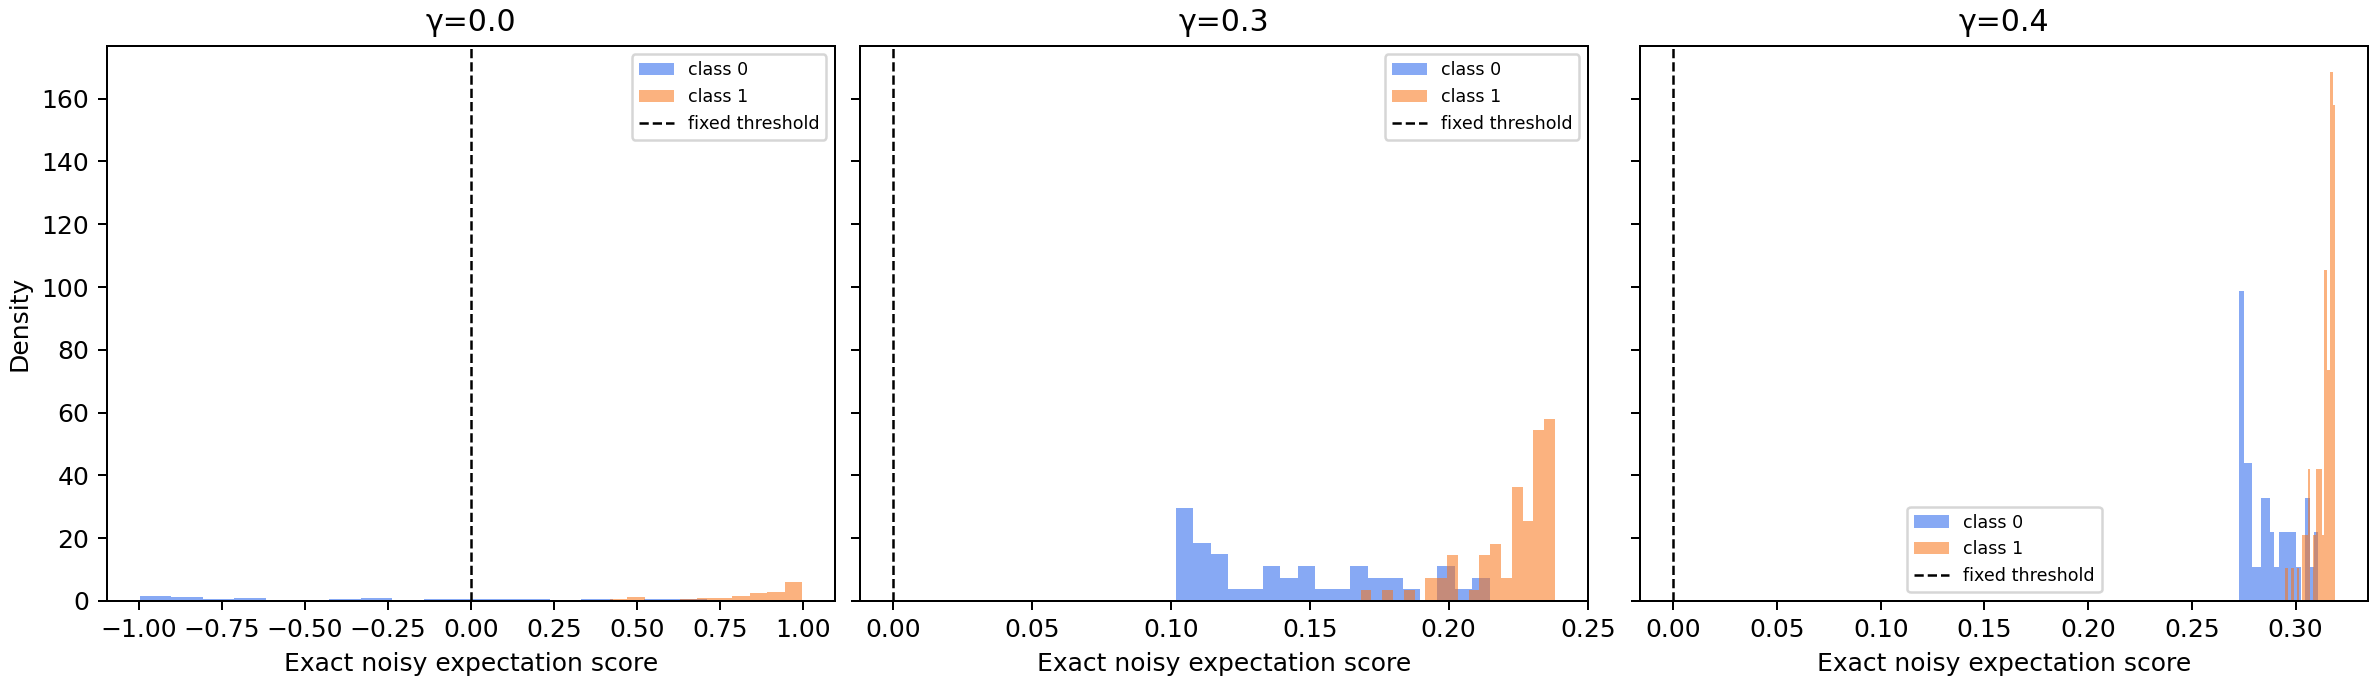
\includegraphics[width=0.48\textwidth]{score_distributions_wdbc.png}
\caption{Secondary unstandardized-PCA exact-expectation accuracy/AUC across composite-noise settings (left) and WDBC score distributions at the selected collapse setting (right).}
\label{fig:supp-exact}
\end{figure*}

\begin{figure*}[t]
\centering
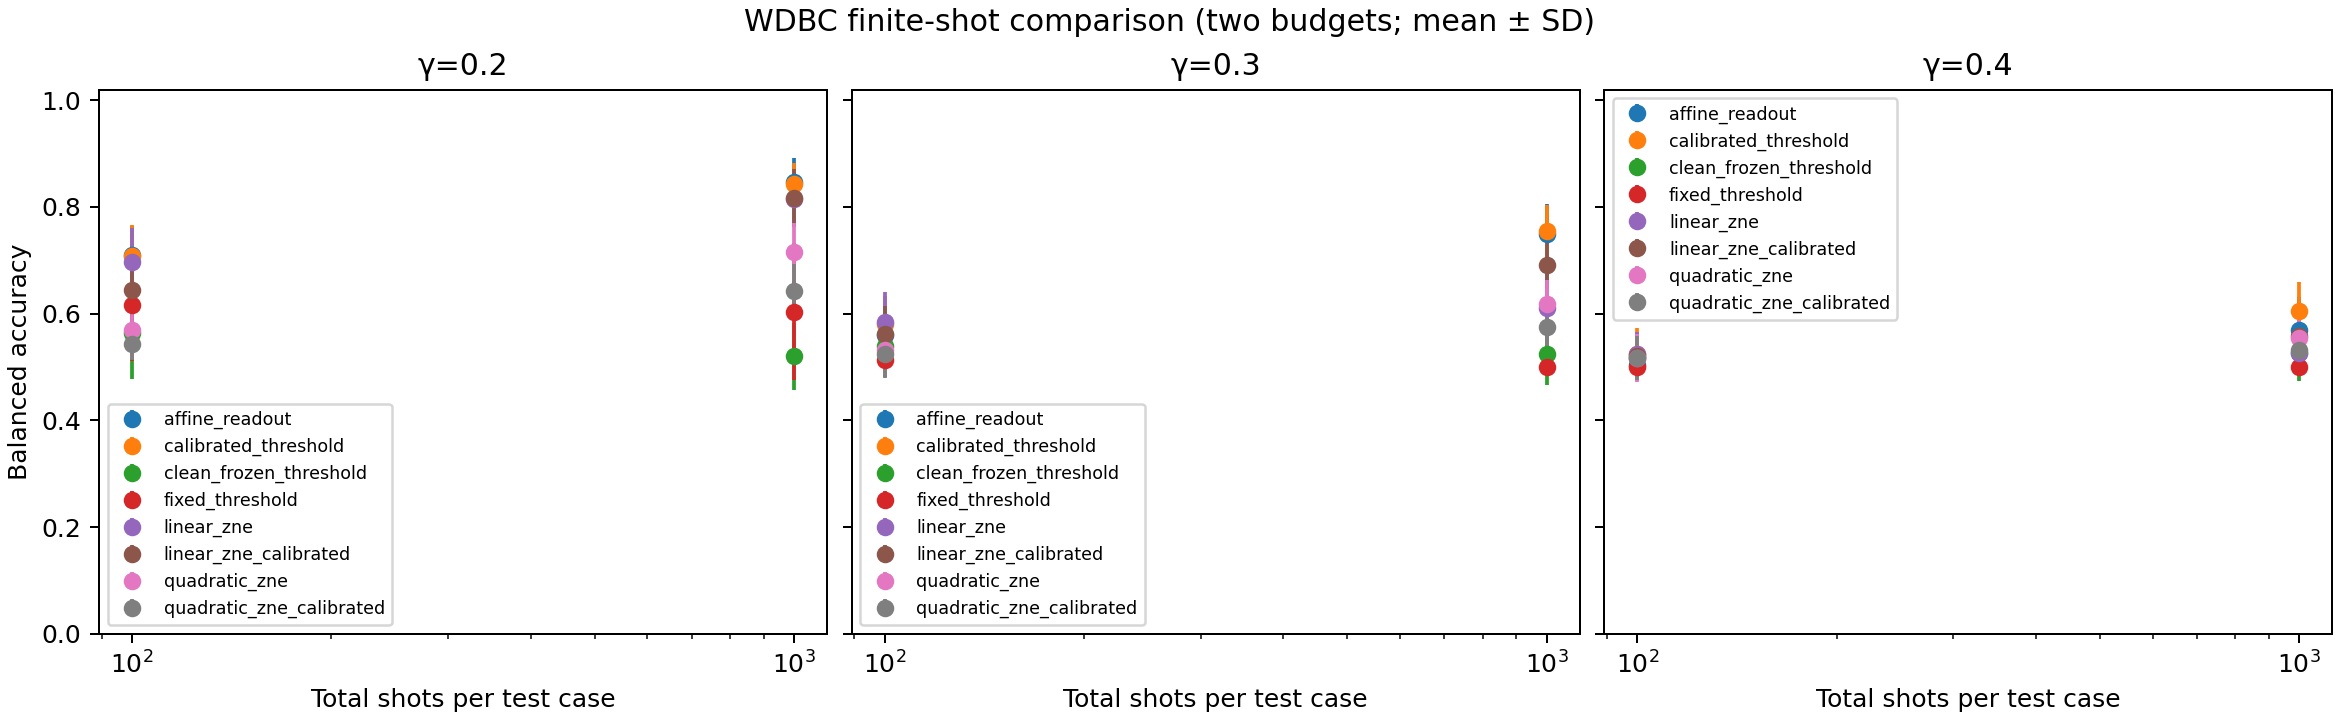
\includegraphics[width=0.48\textwidth]{finite_shots_budget.png}\hfill
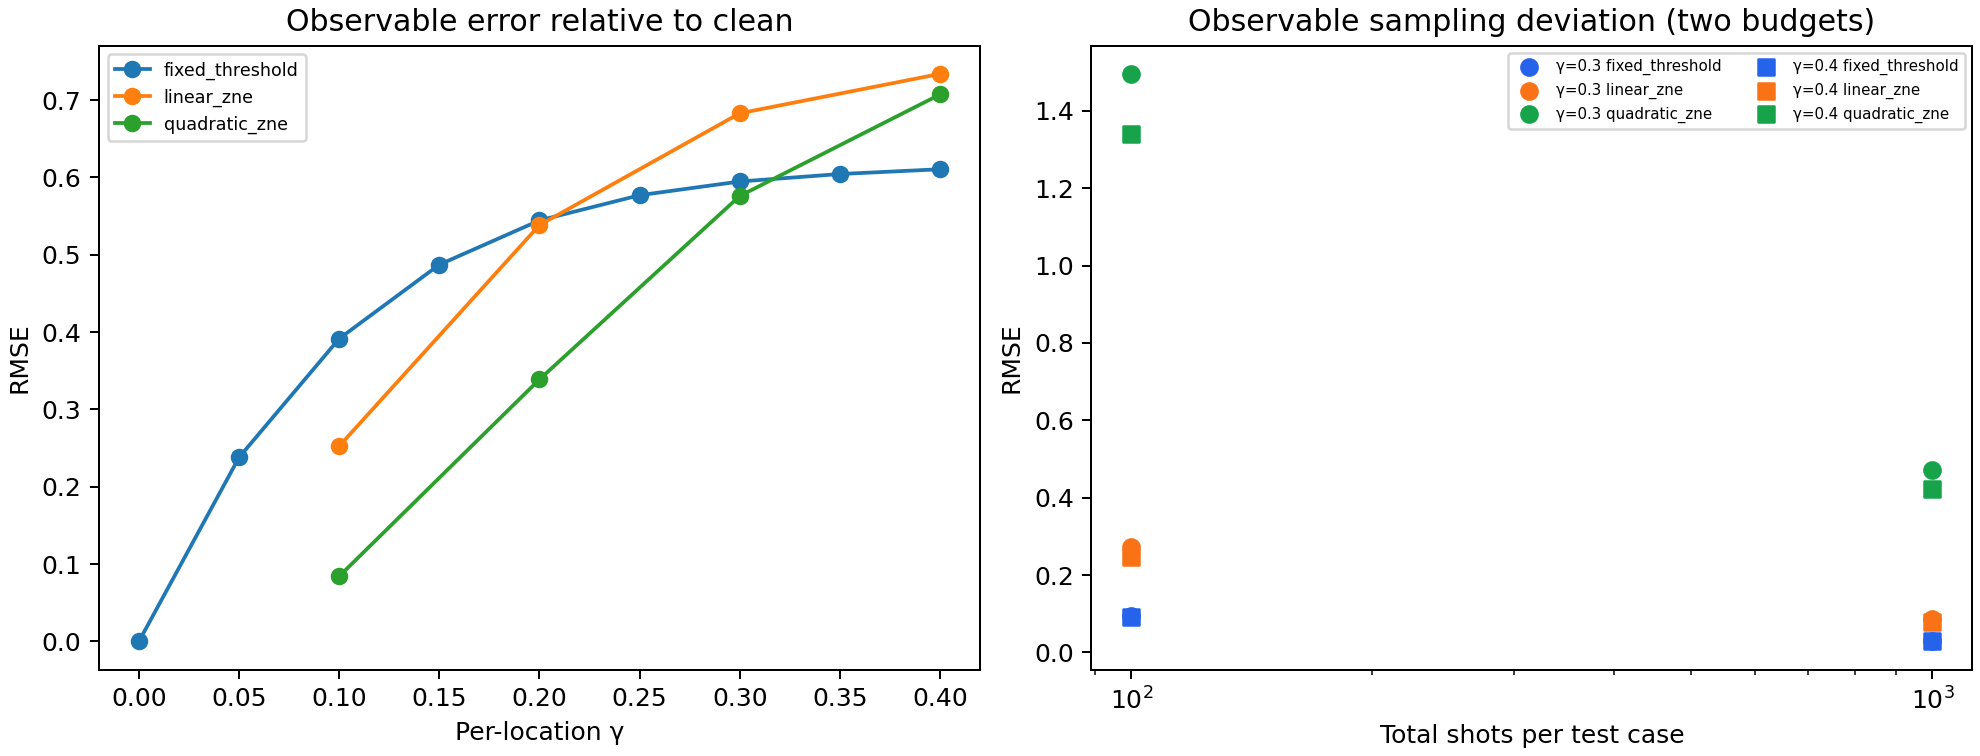
\includegraphics[width=0.48\textwidth]{score_error_decomposition.png}
\caption{Secondary unstandardized-PCA finite-shot balanced accuracy under nominally matched total-shot budgets (realized totals differ by at most 0.443\%), separated by noise level (left); observable estimation error and finite-shot sampling deviation (right; two shot budgets shown as unconnected markers).}
\label{fig:supp-budget}
\end{figure*}

\begin{figure*}[t]
\centering
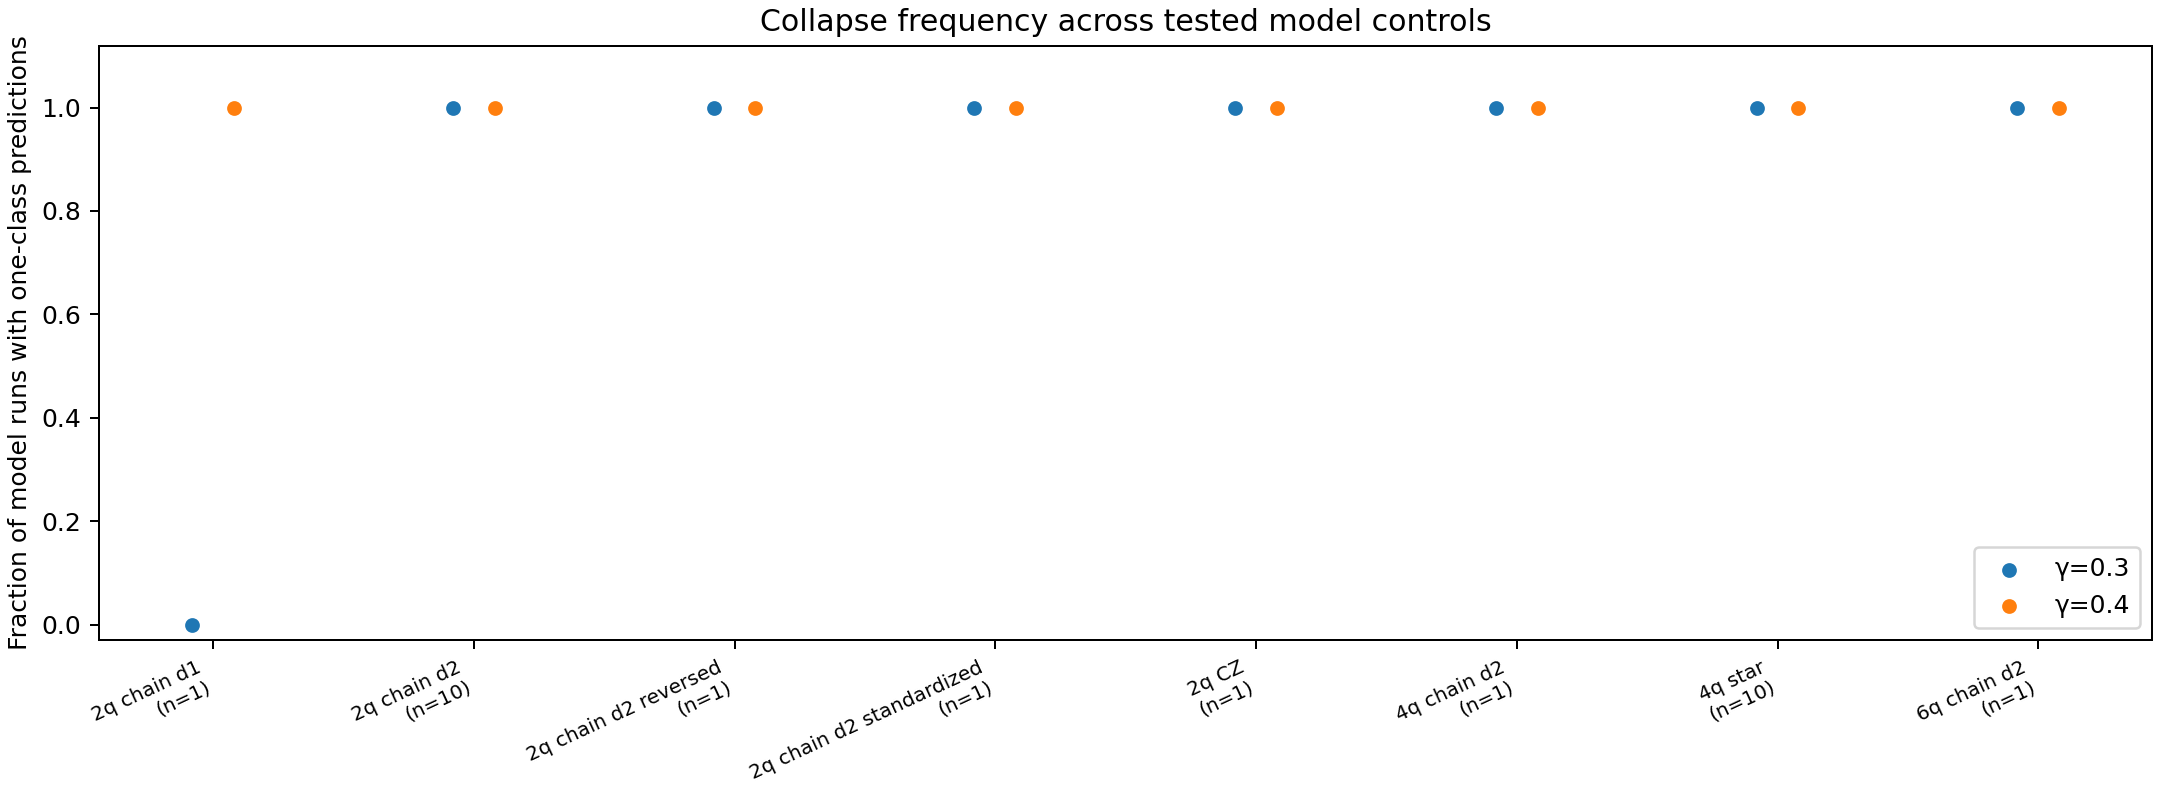
\includegraphics[width=0.92\textwidth]{collapse_controls.png}
\caption{Single-class prediction collapse across architecture, preprocessing, and label-mapping controls. Markers are not connected; labels report the number of model runs supporting each control.}
\label{fig:supp-controls}
\end{figure*}
\end{document}